\documentclass[tikz,border=9pt]{standalone}
\usepackage{amsmath,amssymb}
\usetikzlibrary{arrows.meta,positioning,calc}
\begin{document}
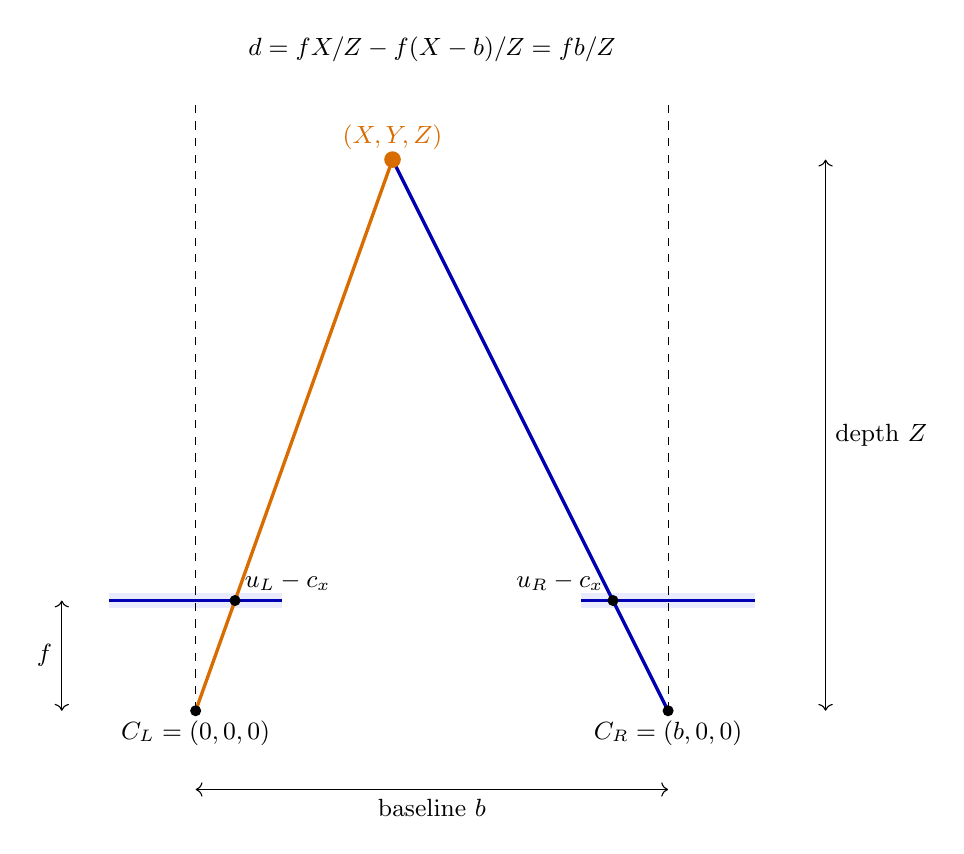
\begin{tikzpicture}[font=\small,arr/.style={-{Stealth},thick},box/.style={draw=blue!55!black,rounded corners,fill=blue!4,align=center,text width=2.9cm,minimum height=1.05cm}]

\coordinate (L) at (0,0);\coordinate (R) at (6,0);\coordinate (P) at (2.5,7);
\fill[blue!8] (-1.1,1.3) rectangle (1.1,1.5);
\fill[blue!8] (4.9,1.3) rectangle (7.1,1.5);
\draw[blue!70!black,thick] (-1.1,1.4)--(1.1,1.4) (4.9,1.4)--(7.1,1.4);
\draw[dashed] (L)--(0,7.8) (R)--(6,7.8);
\draw[very thick,orange!85!black] (L)--(P);
\draw[very thick,blue!70!black] (R)--(P);
\fill (L) circle(2pt) node[below]{$C_L=(0,0,0)$};
\fill (R) circle(2pt) node[below]{$C_R=(b,0,0)$};
\fill[orange!85!black] (P) circle(3pt) node[above]{$(X,Y,Z)$};
\fill (0.5,1.4) circle(2pt) node[above right]{$u_L-c_x$};
\fill (5.3,1.4) circle(2pt) node[above left]{$u_R-c_x$};
\draw[<->] (0,-1)--(6,-1) node[midway,below]{baseline $b$};
\draw[<->] (-1.7,0)--(-1.7,1.4) node[midway,left]{$f$};
\draw[<->] (8,0)--(8,7) node[midway,right]{depth $Z$};
\node at (3,8.4){$d=fX/Z-f(X-b)/Z=fb/Z$};

\end{tikzpicture}
\end{document}
